\documentclass[12pt, twoside]{article}
\usepackage[letterpaper, margin=1in, headsep=0.5in]{geometry}
\usepackage[english]{babel}
\usepackage[utf8]{inputenc}
\usepackage{amsmath}
\usepackage{amsfonts}
\usepackage{amssymb}
\usepackage{tikz}
\usepackage{yhmath}
\usetikzlibrary{quotes, angles}
\usepackage{graphicx}
\usepackage{enumitem}
\usepackage{multicol}

\newif\ifmeta
\metatrue %print standards and topics tags

\title{Regents Geometry}
\author{Chris Huson}
\date{April 2022}

\usepackage{fancyhdr}
\pagestyle{fancy}
\fancyhf{}
\renewcommand{\headrulewidth}{0pt} % disable the underline of the header
\raggedbottom

\fancyhead[LE]{\thepage}
\fancyhead[RO]{\thepage \\ Name: \hspace{4cm} \,\\}
\fancyhead[LO]{BECA / Dr. Huson / Geometry\\* Unit 11: Function transformations\\* 26 April 2022}

\begin{document}
\subsubsection*{11.2 Absolute value function \hfill HSF.BF.B.3}
\begin{enumerate}
\item Part of the parabola $f$: $y=x^2$, is shown below. 
\begin{multicols}{2}
  \begin{enumerate}
    \item Reflect $f$ across the $x$-axis.
    \item Write down the coordinates of $P$.
    \item Mark and label the image $P'$ with its coordinates. \vspace{2cm}
  \end{enumerate}
  \begin{flushright}
    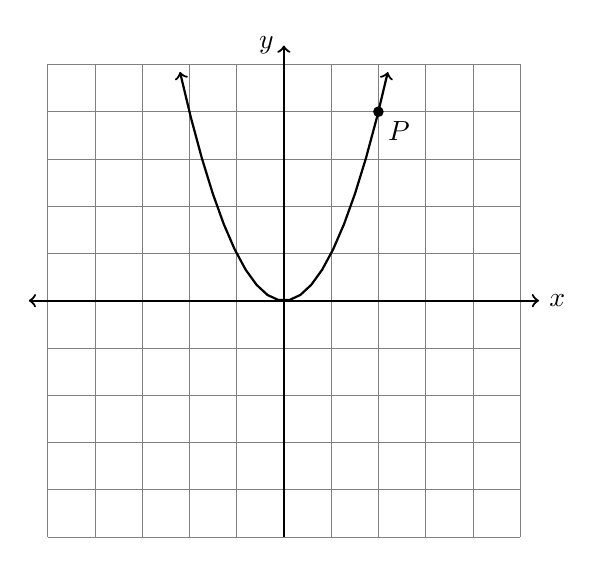
\begin{tikzpicture}[scale=0.6]
    \draw [help lines] (-5,-5) grid (5,5);
    \draw [thick, <->] (-5.4,0) -- (5.4,0) node [right] {$x$};
    \draw [thick, ->] (0,-5)--(0,5.4) node [left] {$y$};  
    \draw [thick,<->,samples=20,domain=-2.2:2.2] plot(\x,\x*\x);
    \draw [fill] (2,4) circle [radius=0.1] node[below right] {$P$};
  \end{tikzpicture}
\end{flushright}
\end{multicols}

\item The line $\overleftrightarrow{RS}$ having the equation $\displaystyle y=\frac{2}{3}x+2$ is shown below.
\begin{multicols}{2}
  \begin{enumerate}
    \item Write down the slope of $\overleftrightarrow{RS}$,\\[0.25cm] $m=$
    \item Write down the $y$-intercept of $\overleftrightarrow{RS}$,\\[0.25cm] $b=$
    \item Dilate $\overleftrightarrow{RS}$ by a scale factor $k=2$ centered at the origin. Mark the images $R'$ and $S'$.
    \item Write down the equation of $\overleftrightarrow{R'S'}$
  \end{enumerate}
  \begin{flushright}
    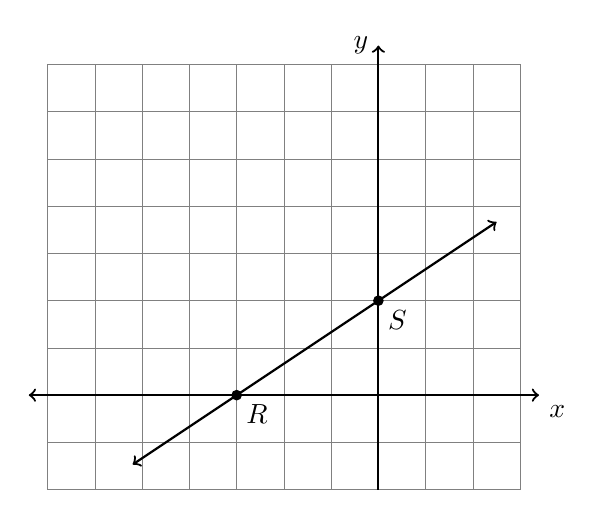
\begin{tikzpicture}[scale=0.6]
      \draw [help lines] (-7,-2) grid (3,7);
      \draw [thick, <->] (-7.4,0) -- (3.4,0) node [below right] {$x$};
      \draw [thick, ->] (0,-2.0)--(0,7.4) node [left] {$y$};
      \draw [thick,<->,samples=20,domain=-5.2:2.5] plot(\x,2/3*\x+2);
      \draw [fill] (-3,0) circle [radius=0.1] node[below right] {$R$};
      \draw [fill] (0,2) circle [radius=0.1] node[below right] {$S$};
    \end{tikzpicture}
  \end{flushright}
\end{multicols}%\vspace{1cm}

\item Write down the translation that would map $g(x)$ onto the parent function $y=x^2$. State your answer in the form $x \rightarrow x-h$, $y \rightarrow y-k$.
\begin{center} 
\begin{tikzpicture}[xscale=1, yscale=1]
  \draw [thick, ->] (-5.2,0) -- (5.4,0) node [below right] {$x$};
  \draw [thick, ->] (0,-0.5)--(0,4.4) node [left] {$y$};
  \foreach \x in {-4,-3,-2,-1,1,2,3,4, 5} \draw (\x cm,3pt)--(\x cm,-3pt) node[below] {$\x$};
  \foreach \y in {1,2,3,4} \draw (3pt,\y cm)--(-3pt,\y cm) node[left] {$\y$};
  \draw [dashed,<->,samples=20,domain=-1.75:1.75] plot(\x,\x*\x);
  \fill (0,0) circle[radius=0.1];
  \draw [thick,<->,samples=20,domain=3.25:6.75] plot(\x,{(\x-5)^2+1});
  \fill (5,1) circle[radius=0.1];
  \node at (5.5,0.5){$(5,1)$};
  \node at (4,3.5){$g(x)$};
\end{tikzpicture}
\end{center}
  
\newpage
Definition: The \emph{absolute value} of a real number is the distance between the number and the origin. (shown here $|A|=3$ and $|B|=4.5$)
\begin{center} 
  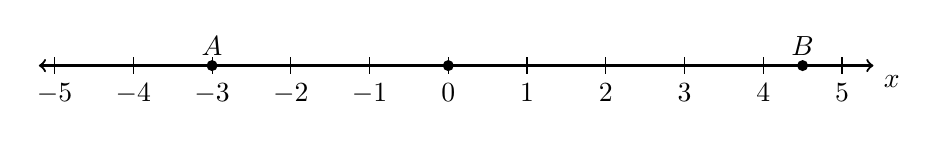
\begin{tikzpicture}[xscale=1, yscale=1]
    \draw [thick, <->] (-5.2,0) -- (5.4,0) node [below right] {$x$};
    \foreach \x in {-5,-4,...,5} \draw (\x cm,3pt)--(\x cm,-3pt) node[below] {$\x$};
    \fill (0,0) circle[radius=0.07];
    \fill (-3,0) circle[radius=0.07]node[above]{$A$};
    \fill (4.5,0) circle[radius=0.07]node[above]{$B$};
  \end{tikzpicture}
  \end{center}
  Equivalently,
\[ |x| =
  \begin{cases}
    x       & \quad \text{if } x \geq 0\\
    -x  & \quad \text{if } x < 0
  \end{cases}
\]

\item Complete the t-table for the function $f$: $y=|x|$, plot the points, and draw $f$ as a smooth curve.
  \begin{center} 
  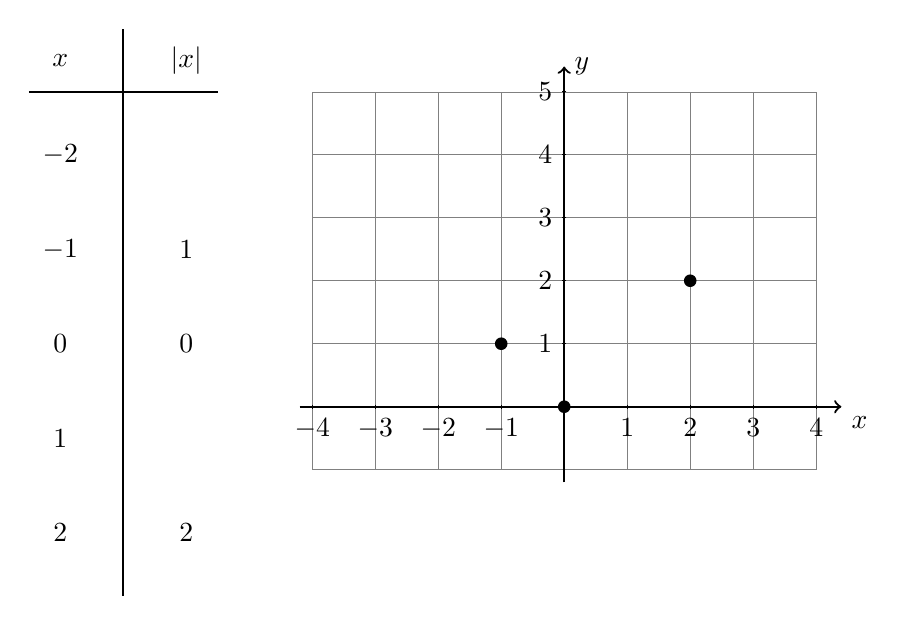
\begin{tikzpicture}[scale=0.8]
    \draw [help lines] (-4,-1) grid (4,5);
    \draw [thick, ->] (-4.2,0) -- (4.4,0) node [below right] {$x$};
    \draw [thick, ->] (0,-1.2)--(0,5.4) node [right] {$y$};
    \foreach \x in {-4,-3,-2,-1,1,2,3,4} \draw (\x cm,1pt)--(\x cm,-1pt) node[below] {$\x$};
    \foreach \y in {1,2,3,4,5} \draw (1pt,\y cm)--(-1pt,\y cm) node[left] {$\y$};
    \draw [thick] (-7,-3) -- (-7,6);
    \draw [thick] (-8.5,5) -- (-5.5,5);
    %\node at (-7,7){$f(x)$};
    \node at (-8,5.5){$x$}; \node at (-6,5.5){$|x|$};
    \node at (-8,4){$-2$};
    \node at (-8,2.5){$-1$}; \node at (-6,2.5){$1$};
    \node at (-8,1){$0$};  \node at (-6,1){$0$};
    \node at (-8,-0.5){$1$};
    \node at (-8,-2){$2$}; \node at (-6,-2){$2$};
    %\fill (-2,4) circle[radius=0.1];
    \fill (-1,1) circle[radius=0.1];
    \fill (0,0) circle[radius=0.1];
    %\fill (1,1) circle[radius=0.1];
    \fill (2,2) circle[radius=0.1];
  \end{tikzpicture}
  \end{center}

\item The function $g: y = |x-2|+3$ is plotted below as a solid line. What translation would map $g$ onto the parent function (dotted)?  State your answer in the form $x \rightarrow x-h$, $y \rightarrow y-k$.
\begin{center} 
\begin{tikzpicture}[xscale=1.0, yscale=1]
  \draw [thick, ->] (-5.2,0) -- (5.4,0) node [below right] {$x$};
  \draw [thick, ->] (0,-0.5)--(0,4.4) node [left] {$y$};
  \foreach \x in {-4,-3,-2,-1,1,2,3,4, 5} \draw (\x cm,3pt) -- (\x cm,-3pt) node[below] {$\x$};
  \foreach \y in {1,2,3,4} \draw (3pt,\y cm) -- (-3pt,\y cm) node[left] {$\y$};
  \draw [dashed,<->,samples=20,domain=-1.75:1.75] plot(\x,abs{\x});
  \fill (0,0) circle[radius=0.1];
  \draw [thick,<->,samples=50,domain=0:4] plot(\x,abs{(\x-2)}+3);
  \fill (2,3) circle[radius=0.1];
  \node at (2.5,2.5){$(2,3)$};
  \node at (4,4.5){$g(x)$};
\end{tikzpicture}
\end{center}

\end{enumerate}
\end{document}
  